\documentclass[a4j]{jsarticle}
\setlength{\topmargin}{-20.4cm}
\setlength{\oddsidemargin}{-10.4mm}
\setlength{\evensidemargin}{-10.4mm}
\setlength{\textwidth}{18cm}
\setlength{\textheight}{26cm}

\usepackage[top=15truemm,bottom=20truemm,left=20truemm,right=20truemm]{geometry}
\usepackage[latin1]{inputenc}
\usepackage{amsmath}
\usepackage{amsfonts}
\usepackage{amssymb}
\usepackage[dvipdfmx]{graphicx}
\usepackage[hang,small,bf]{caption}
\usepackage[subrefformat=parens]{subcaption}
\usepackage[dvipdfmx]{color}
\usepackage{listings}
\usepackage{listings,jvlisting}
\usepackage{geometry}
\usepackage{framed}
\usepackage{color}
\usepackage[dvipdfmx]{hyperref}
\usepackage{ascmac}
\usepackage{enumerate}
\usepackage{tabularx}
\usepackage{cancel}
\usepackage{scalefnt}
\usepackage{overcite}
\usepackage{otf}
\usepackage{multicol}
\usepackage[geometry]{ifsym}

\renewcommand{\figurename}{Fig.}
\renewcommand{\tablename}{Table }

\lstset{
basicstyle={\ttfamily},
identifierstyle={\small},
commentstyle={\smallitshape},
keywordstyle={\small\bfseries},
ndkeywordstyle={\small},
stringstyle={\small\ttfamily},
frame={tb},
breaklines=true,
columns=[l]{fullflexible},
xrightmargin=0zw,
xleftmargin=3zw,
numberstyle={\scriptsize},
stepnumber=1,
numbersep=1zw,
lineskip=-0.5ex
}

% キャプション後ろのダブルコロンを消す
\makeatletter
\newenvironment{tablehere}
{\def\@captype{table}}

\newenvironment{figurehere}
{\def\@captype{figure}}

\long\def\@makecaption#1#2{%
  \vskip\abovecaptionskip
  \iftdir\sbox\@tempboxa{#1\hskip1zw#2}%
    \else\sbox\@tempboxa{#1 #2}%
  \fi
  \ifdim \wd\@tempboxa >\hsize
    \iftdir #1\hskip1zw#2\relax\par
      \else #1 #2\relax\par\fi
  \else
    \global \@minipagefalse
    \hbox to\hsize{\hfil\box\@tempboxa\hfil}%
  \fi
  \vskip\belowcaptionskip}
\makeatother

% タイトル
\makeatletter
\def\@maketitle
{
\begin{center}
{\LARGE \@title \par}
\end{center}
\begin{flushright}
{\large \@date 報告書 No.30}\\
{\large M2 \@author}
\end{flushright}
\par\vskip 1.5em
}
\makeatother

\author{来代 勝胤}
\title{令和4年度 6月 第3週 報告書}
\date{2022/6/20}

\begin{document}
\columnseprule=0.1mm
\maketitle

\begin{figure*}[htbp]
  \begin{center}
    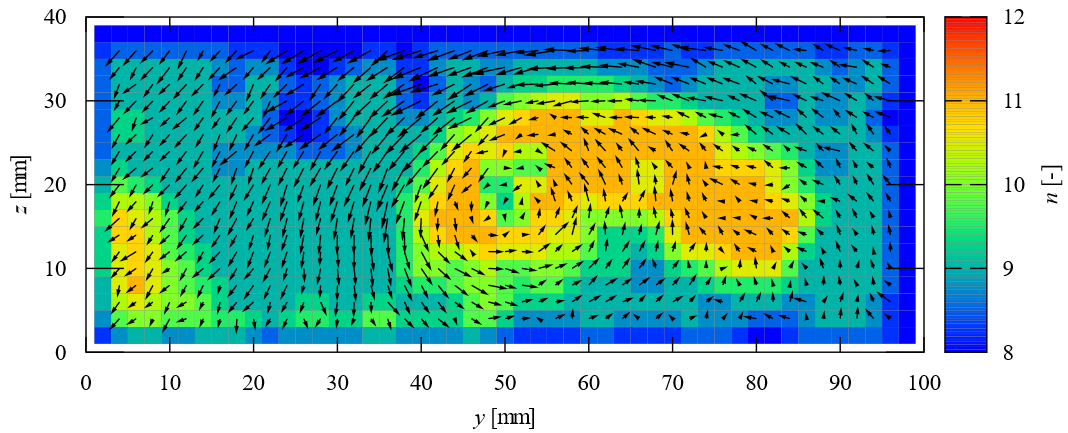
\includegraphics[width=150mm]{../images/velocity_and_vorticity.png}
    \caption{Velocity vectors and vorticity of delta wake}
  \end{center}
\end{figure*}

\begin{multicols*}{2}
  \section*{報告内容}
  \begin{enumerate}[1.]
    \item 枚数差の組み合わせ変更(続)
    \item 数値シミュレーション
    \item 来週の予定
  \end{enumerate}
  \section{枚数差の組み合わせ変更(続)}
  先週に引き続き,枚数差の組み合わせによる差異の検討を行った.
  Fig.1 について,最大の相間係数をとる組み合わせを選択して
  速度場を表現した結果を示す.
  結果より,渦中心の対応枚数差$n$が大きくなっていることから
  主流方向速度が低下していることがわかる.
  また,渦中心から離れるごとに$n$の値が小さくなっており,
  円状に分布していることからも妥当性の高い結果だと考えられる.
  したがって,場所によって対応枚数差を変更する必要があることがわかった.

  \section{数値シミュレーション}
  数値シミュレーションによる計測アルゴリズム評価について,
  Fig.2,Fig.3 に1枚当たりの粒子数$n$と角速度$\omega$の関係について,
  RMSE率の算出結果を示す.

  \columnbreak
  \begin{figurehere}
    \footnotesize
    \begin{center}
      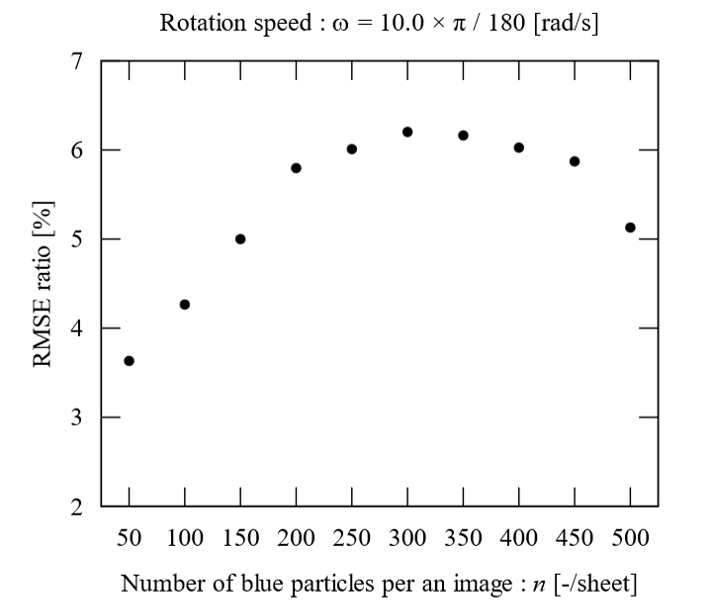
\includegraphics[width=55mm]{../images/error-1.png}
      \caption{RMSE ratio due to difference in $n$}
      \vskip \baselineskip
      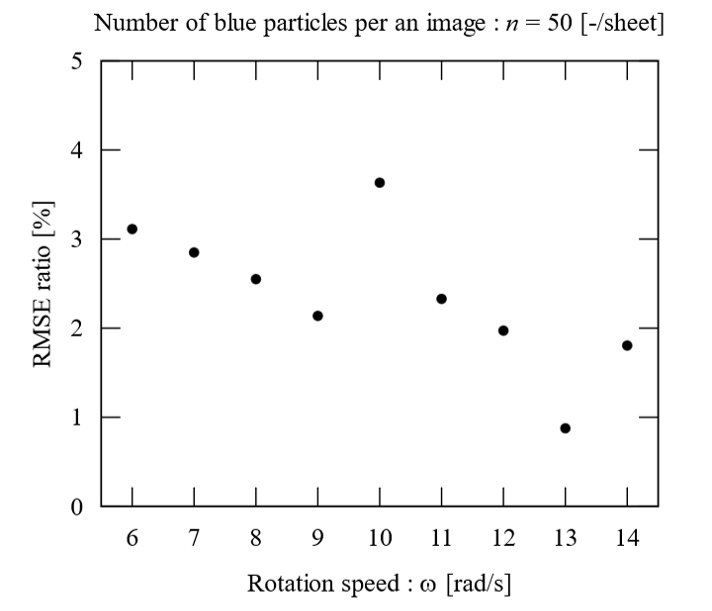
\includegraphics[width=55mm]{../images/error-2.png}
      \caption{RMSE ratio due to difference in $\omega$}
    \end{center}
  \end{figurehere}
  \section{来週の予定}
  \begin{itemize}
    \item ISTP-33 原稿作成
    \item 共同研究報告会の資料作成
  \end{itemize}
\end{multicols*}

\end{document}